\documentclass[11pt,a4paper]{jsarticle}                    % fir platex
%\documentclass[11pt,a4paper,uplatex]{ujreport} 	% for uplatex
%
\usepackage{amsmath,amssymb}
\usepackage{bm}
\usepackage{graphicx}
\usepackage{ascmac}
\usepackage{float}
%
\setlength{\textheight}{40\baselineskip}
\addtolength{\textheight}{\topskip}
\setlength{\voffset}{-0.2in}
\setlength{\topmargin}{0pt}
\setlength{\headheight}{0pt}
\setlength{\headsep}{0pt}

\setlength{\textwidth}{\paperwidth}     % ひとまず紙面を本文領域に
\setlength{\oddsidemargin}{-5.4truemm}  % 左の余白を20mm(=1inch-5.4mm)に
\setlength{\evensidemargin}{-5.4truemm} % 
\addtolength{\textwidth}{-40truemm}     % 右の余白も20mmに
%
\newcommand{\divergence}{\mathrm{div}\,}  %ダイバージェンス
\newcommand{\grad}{\mathrm{grad}\,}  %グラディエント
\newcommand{\rot}{\mathrm{rot}\,}  %ローテーション
%
\title{脳波解析のための数学シリーズ\\
統計編}
\author{後藤 優仁}
\date{\today}
\begin{document}
\maketitle

\newpage
%
%
\tableofcontents
\newpage
\section{はじめに}
 統計処理とは, 実際に実験やアンケートを通して集めたデータを解釈する際に必要になる処理です. 論文を読むためにも必須, というか一番大事な項目なので頑張りましょう. analysisの様々な処理を行った結果,実験で計測した脳波を何らかの形で解釈しやすいようなデータに変形する事が出来ました.つまり解析をしました.次に必要なのは,この解析で得られたデータを解釈する行程です.ここで必要になるのが統計的な処理ですね.個人的には楽しくないですが,仕方ないのでやっていきましょう.\\
  また,結局脳の計算をモデル化しようとか発展的な議論をしていこうと思った時にはここら辺が非常に重要になってきます.先に勉強しておくとだいぶ後が楽だと思いますが,何に役立つのか分からないとモチベは上がらないし勉強できないのは自分も痛いほど分かるので,逆に先にadvanced.pdfとかでチラ見してくるのも良いかもしれませんね.\\
  特に,今はまだ追加できていませんがベイズ統計は勉強しておくべきです.勉強するだけで色々と広がっていきます.本当に.
 
 \newpage
 
 
\section{確率分布}
\subsection{確率分布と確率密度関数}
確率とは, 起こりうる全体の事象のうち, ある事象がどれくらいの割合で起こるのかを表します. 確率分布とは, 起こりうる事象それぞれの確率がどのような分布をしているかです. \\
確率密度関数とは, 実際に確率分布をプロット(横軸に事象, 縦軸に確率)した際に現れる分布の形を表現する関数の事です. 場合によっては事象は離散分布になったりするため,その場合はこの分布を連続と見立てて確率密度関数が定義されます.\\

\subsection{一様分布/ベルヌーイ分布/2項分布/ポアソン分布}
まずは簡単な分布から見て, 徐々に複雑なものを見ていきます. 今回は脳の数学であまり使わない気がするやつらはまとめて雑に確認します.\\
\subsubsection{一様分布}
例えばサイコロを振った時に出る目の確立分布を考えると, 当然6つの事象それぞれがすべて$\frac{1}{6}$で表せるため, プロットすると以下のようになります.\\
\begin{figure}[H]
\label{im:uniform}
  \centering
  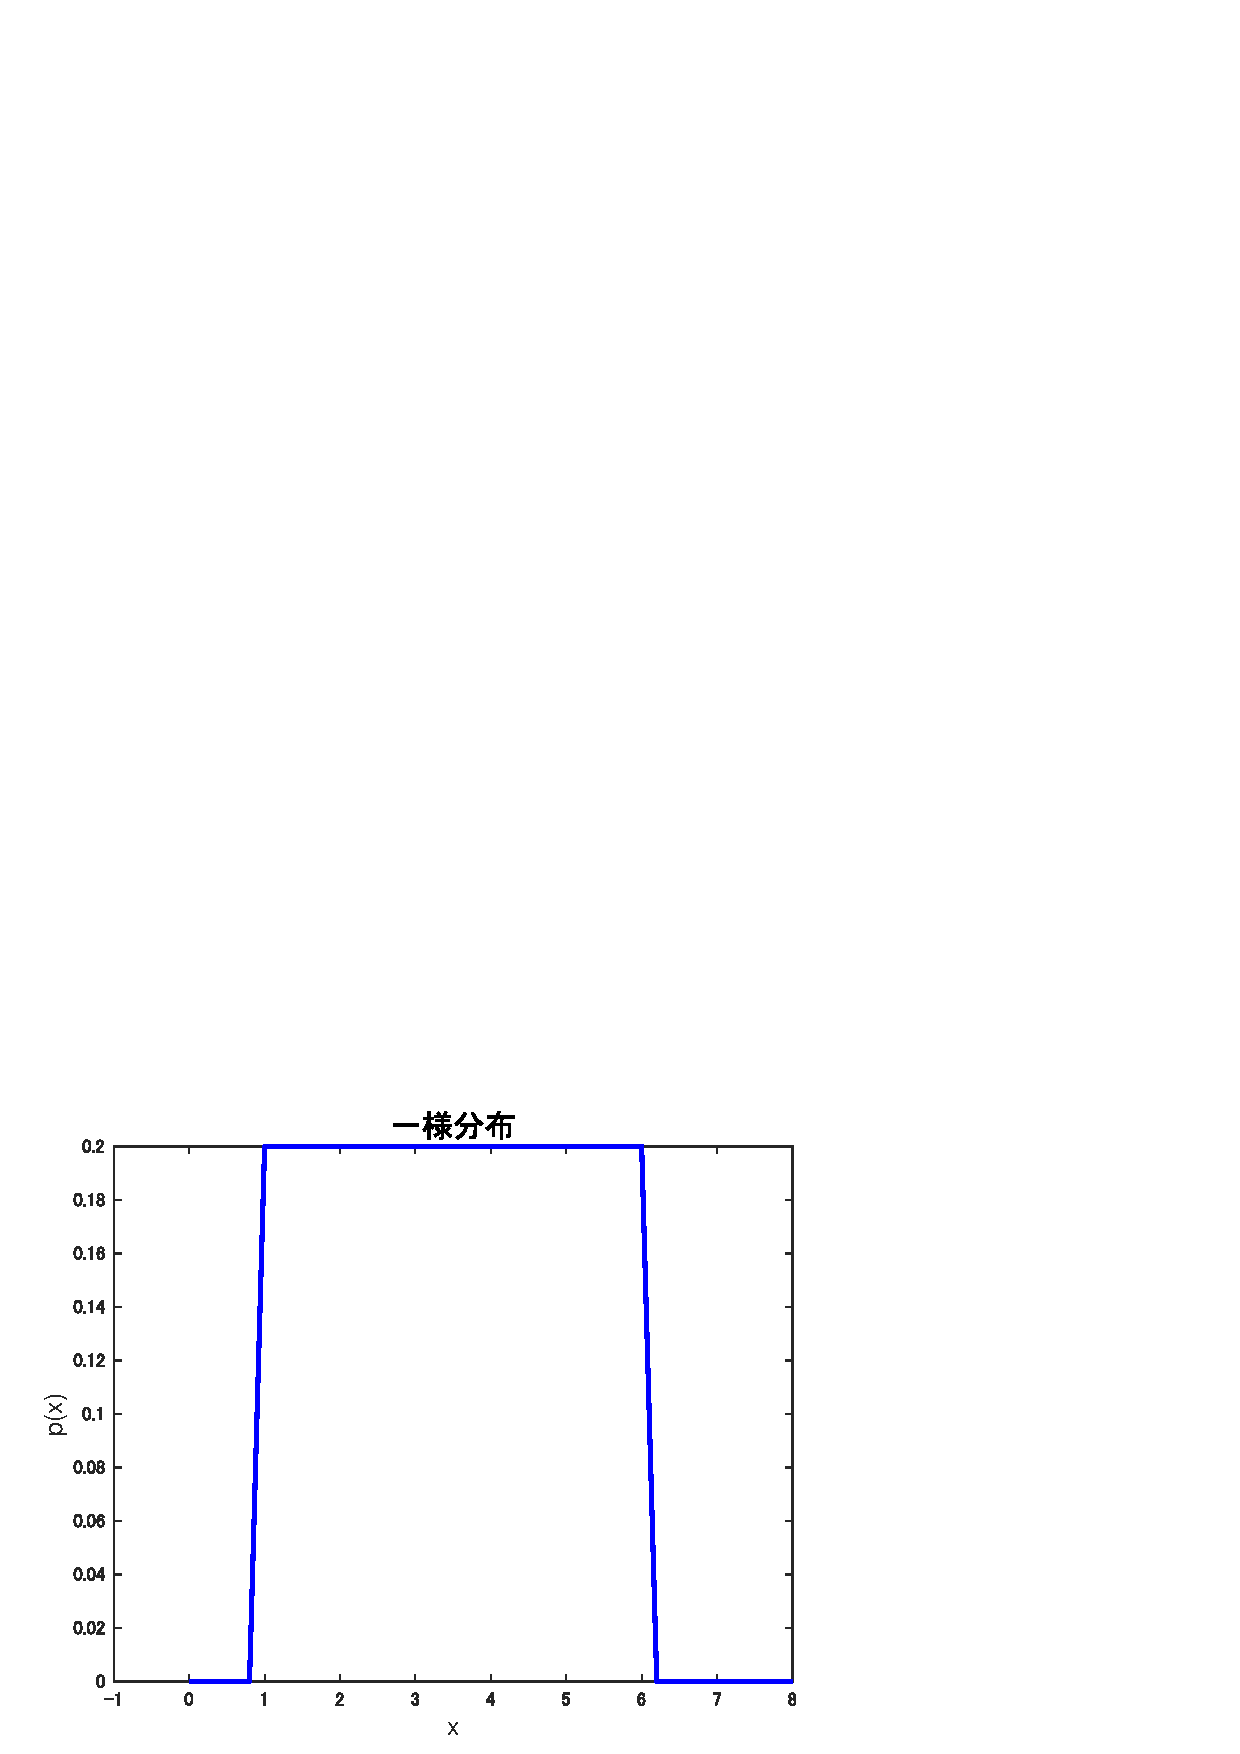
\includegraphics[width=120mm,bb=0 0 432 288]{figures/uniform.png}
  \caption{サイコロの確立分布(一様分布)}
\end{figure}

一様分布は確率密度関数を定義するまでもないのですが, 勉強のためにあえてやるとすると以下のようになります. まずさいころの例だとそれぞれの目が出てくる確率はこうですね.

\begin{eqnarray}
\label{eq:uniform}
f(x) = \frac{1}{6} (1 \leq X \leq 6)
\end{eqnarray}

定義域が0から6で, いずれの点においても$\frac{1}{6}$の確立で目がでるよってことですね. 簡単です. また確率を考える際, 式(\ref{eq:uniform})のように左辺の$(x)$と右辺定義域内にいる$(X)$で使い分けがなされます. $X$は確率変数を表し, 実際の値は取りません. 観測されて確定した時には$x$として表現されます. 今回の$X$と$x$の関係は

\begin{eqnarray}
X = [x_1, x_2, x_3, x_4, x_5, x_6]
\end{eqnarray}
のような感じです. \\
\\
より一般には離散一様分布に従う変数の確率関数は,Nを変数が取りうる値(さいころの目=6)として,

\begin{eqnarray}
P(X=x) = \frac{1}{N} \qquad (x=1,2,...,N)
\end{eqnarray}
となります.これはさすがに良いですよね.次.\\
離散一様分布の期待値と分散は以下です.\\

\begin{eqnarray}
\begin{split}
\mathbb{E}(X) &= \sum_{k=1}^N{kP(X=k)}\\
&=\sum_{k=1}^N{k\frac{1}{N}}\\
&= \frac{(1+N)N}{2}\frac{1}{N}\\
&= \frac{1+N}{2}
\end{split}
\end{eqnarray}

\begin{eqnarray}
\begin{split}
\mathbb{V}(X) &= \mathbb{E}(X^2) - \mathbb{E}(X)^2\\
&= \sum_{k=1}^N k^2 \frac{1}{N} - {(\frac{1+N}{2})}^2\\
&= \frac{1}{N}N\frac{(N+1)(2N+1)}{6}-\frac{(N+1)^2}{4}\\
&= \frac{N^2-1}{12}
\end{split}
\end{eqnarray}
\\
一見複雑?な気もするかもしれませんが,普通に計算してみればわかるとおもいます.ほら,「1から100までの数の和は?」みたいな問題って工夫して暗算出来ましたよね?どうやるんでしたっけ.\\
\\
連続一様分布については確率密度関数は以下のようになります.

\begin{eqnarray}
f(x) = 
\left\{
    \begin{array}{l}
      \frac{1}{b-a} \qquad \qquad  (a \leq X \leq b) \\
      0  \qquad \qquad \qquad(otherwise)
    \end{array}
  \right.
\end{eqnarray}

これは面積で考えると分かりやすいかも.確率密度関数は積分すると1にならないといけません.b-aは定義域なので,つまり面積でいうところの横の長さです.縦の長さはそれぞれの値が観測される確率,つまり$f(x)$ですよね?\\
そう,なので定義の$f(x)$を定義域で積分すると1になります.当たり前の事なのですが,確率密度関数の考え方にいまいち慣れていない人ように丁寧に言いました.以下はこのような話は省略します.\\
とにかく,積分すると1になるのが確率密度関数です.


平均$\mathbb{E}(X)$及び分散$\mathbb{V}(X)$は

\begin{eqnarray}
\mathbb{E}(X) = \frac{a+b}{2}\\
\mathbb{V}(X) = \frac{(b-a)^2}{12}
\end{eqnarray}

一応,期待値くらいは証明もしておきます.でもまあ簡単です.

\begin{eqnarray}
\begin{split}
\mathbb{E}(X)  &= \int_{-\infty}^{\infty} xf(x) dx \\
&= \int_{-\infty}^{a} xf(x) dx + \int_{a}^{b} xf(x) dx + \int_{b}^{\infty} xf(x) dx \\
&= 0 + \int_{a}^{b} x\frac{1}{b-a} dx + 0\\
&= \frac{1}{b-a}\left[\frac{x^2}{2}\right]_a^b\\
& = \frac{b-a}{2}
\end{split}
\end{eqnarray}

\subsubsection{ベルヌーイ分布}
ベルヌーイ分布は, 1か0かです. ある事が起きるか起きないか, 成功するかしないかなどの2値分類ですね. 超簡単です!!\\

\begin{figure}[H]
\label{im:bernoulli}
  \centering
  \includegraphics[width=120mm,bb=0 0 432 288]{figures/bernoulli.png}
  \caption{ベルヌーイ分布}
\end{figure}
今回は1:1の図になっていますが, もちろん1:5くらいの割合になる事もあります. たとえばサイコロで1が出るか出ないかとか. 以上.\\
\\
関数はこんな感じかな
\begin{eqnarray}
f(x)=
  \left\{
    \begin{array}{l}
      p \qquad \qquad \qquad (x = 1) \\
      q(=1-p)  \qquad (x=0)
    \end{array}
  \right.
\end{eqnarray}

平均$\mathbb{E}(X)$及び分散$\mathbb{V}(X)$は

\begin{eqnarray}
\mathbb{E}(X) = p\\
\mathbb{V}(X) = pq
\end{eqnarray}

です. 興味ないので証明とかやりません. 僕も知らない.
\subsubsection{2項分布}
2項分布は「同じことを何回も繰り返した時, ある事柄が何回おこるか」の確立分布です. こいつは式を見れば早いですね.

\begin{eqnarray}
\label{eq:binomial}
f(x) = {}_n\mathrm{C}_x p^x(1-p)^{n-x}
\end{eqnarray}

式(\ref{eq:binomial})の右辺左側にある${}_n\mathrm{C}_x p^x$は, 確率pで起こる事象Aが, 全体nのうちx回でたという意味で, 右側の$(1-p)^{n-x}$は確率(1-p)で, Aが起きなかった回数が(n-x)回出たという意味です.\\
これらを掛け合わせているので, 何回当たって何回外れたかを表す式ですね.

\begin{figure}[H]
\label{im:bernoulli}
  \centering
  \includegraphics[width=120mm,bb=0 0 432 288]{figures/binomial.png}
  \caption{ベルヌーイ分布}
\end{figure}

平均$\mathbb{E}(X)$及び分散$\mathbb{V}(X)$は

\begin{eqnarray}
\mathbb{E}(X) = np\\
\mathbb{V}(X) = np(1-p)
\end{eqnarray}

です. 興味ないので証明とかやりません. 僕も知らない.

\subsubsection{ポアソン分布}
ポアソン分布は「稀な事象が一定時間内にどれくらい起きるか」です.\\
たとえば, ある月にある地域で起きた交通死亡事故の件数とかです. 修羅の国やグンマ―, あるいは名古屋でもない限り, 普通は0か多くて2件とかですよね.\\
\\
確率密度関数は以下です.
\begin{eqnarray}
f(x) = \frac{\lambda^x}{x!}e^{-\lambda}
\end{eqnarray}

平均$\mathbb{E}(X)$及び分散$\mathbb{V}(X)$は

\begin{eqnarray}
\mathbb{E}(X) = \lambda\\
\mathbb{V}(X) = \lambda
\end{eqnarray}

です. こいつの場合, 平均も分散も同じ定数$\lambda$なので, こいつの値だけで形が決まります. $\lambda$がどんな値なのか, どうやって決まるのかは知りません. 使う事があれば足します.\\

\begin{figure}[H]
\label{im:poisson}
  \centering
  \includegraphics[width=120mm,bb=0 0 432 288]{figures/poisson.png}
  \caption{ポアソン分布}
\end{figure}

\subsection{正規分布}
\subsubsection{正規分布とは}
さて本題です. 数ある確率分布の中でも抜きんでて重要な分布, 正規分布, またの名をガウス分布です. 世の中の多くの事象がこの分布に従っていて, また従っていると仮定して統計的処理がされています. 今後の統計学の基礎になるのでしっかり理解しましょう.\\
\\
正規分布は, 平均$\mathbb{E}(X)$が母集団の平均$μ$と等しく, 分散$\mathbb{V}(X)$も母集団の分散$\sigma ^2$と等しくなる分布で, 確率密度関数は以下になります.

\begin{eqnarray}
\label{eq:normal}
f(x) = \frac{1}{\sqrt{2\pi\sigma^2}}e^{-\frac{(x-\mu)^2}{2\sigma^2}}
\end{eqnarray}

いや, うん. 分かります. やばそうですよね. \\
ただまぁ, なんでこんな殺意高めな式になるのかは正規分布のグラフを見れば理解できます. 母集団の平均が50, 標準偏差20の正規分布だとこうなります.

\begin{figure}[H]
\label{im:normal}
  \centering
  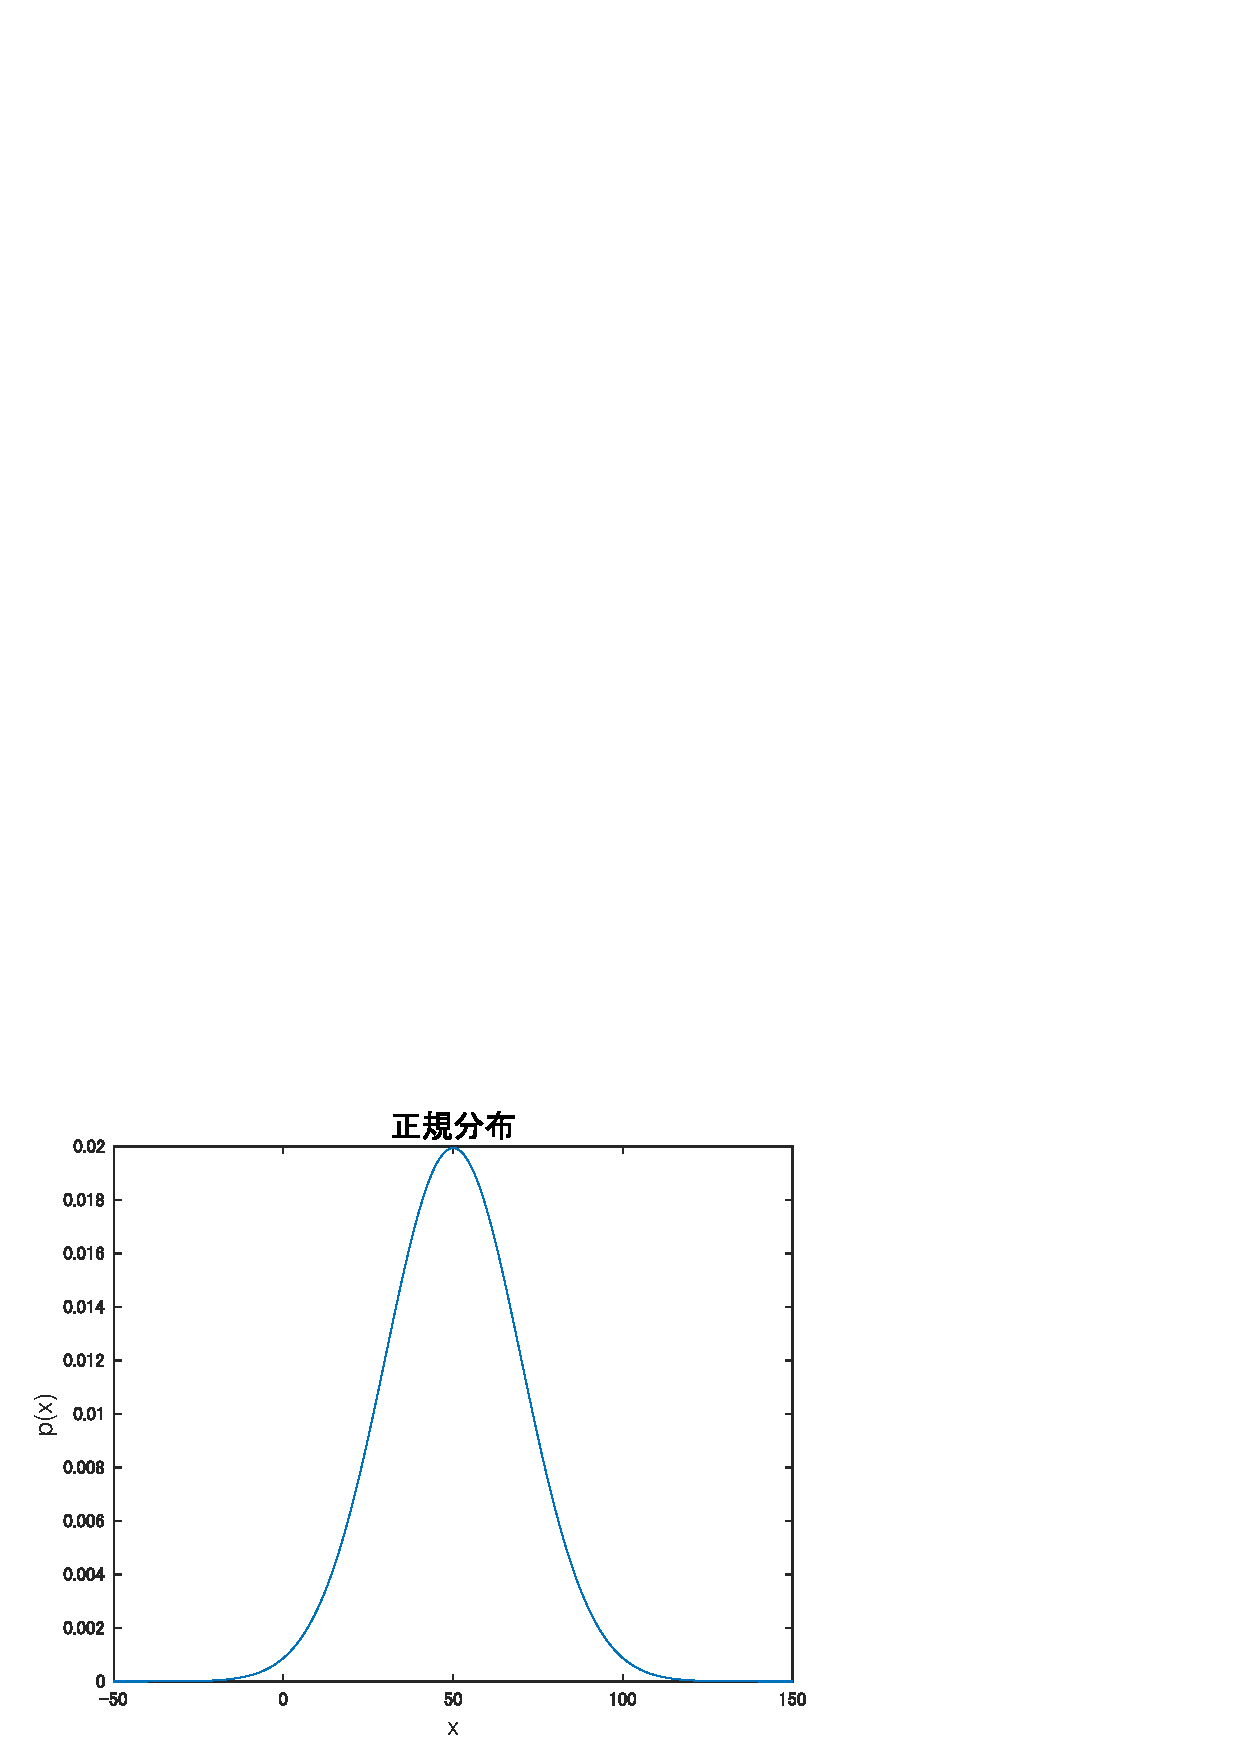
\includegraphics[width=120mm,bb=0 0 432 288]{figures/normal.png}
  \caption{正規分布}
\end{figure}

定義通り, 確率変数の平均も50, 分散も400(20の二乗)になっていますね!!これが正規分布です. 綺麗ですね.\\
\\
\subsubsection{確率密度関数の導出}
さて, 式(\ref{eq:normal})の解説です. まずややこしいとこを全て消し飛ばし, 以下のように変形しましょう. 

\begin{eqnarray}
\label{eq:normal2}
f(x) = e^{-x^2}
\end{eqnarray}

\begin{figure}[H]
\label{im:normal}
  \centering
  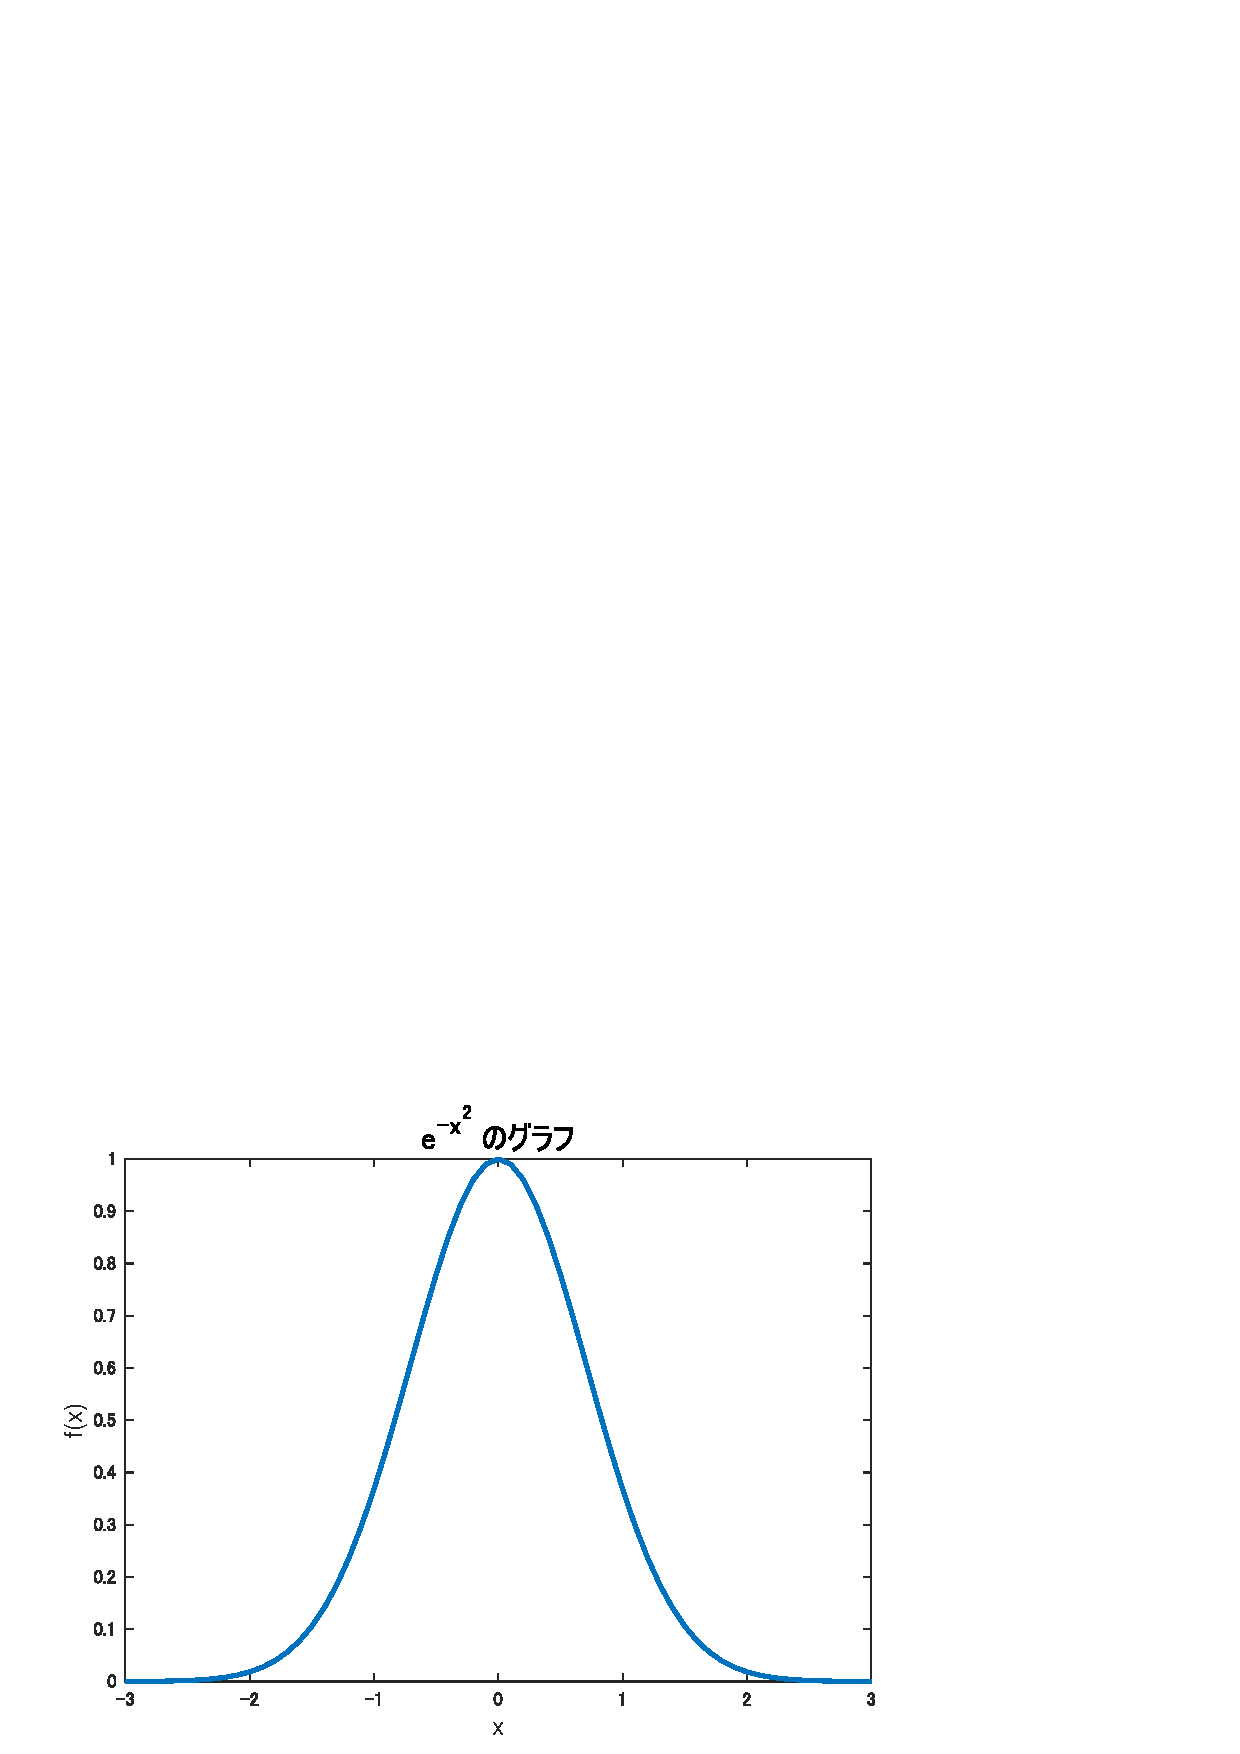
\includegraphics[width=120mm,bb=0 0 432 288]{figures/normal2.png}
  \caption{式(\ref{eq:normal2})の図}
\end{figure}

この関数の説明はいりませんね? 指数関数の二乗の負版です.\\
まず, 世の中の多くの事象は平均値を取る確率が一番大きく, 平均値から離れるにつれその値を取る確率は小さくなることが知られています. んで, これをどう数式で表現すれば良いかと悩んだ末考えだされたのが正規分布関数だと思ってください.\\
そうすると, とりあえず釣り鐘型の関数が欲しいという事で式(\ref{eq:normal2})を考えました. 実際これでほぼ完成です.\\
ただ, これは任意定数がないため平均が0, 分散(幅)も一定ですね. これでは実用できません. そこで任意定数を導入し, 平均値と分散を可変にします. 平均値, つまりこのグラフの頂点の位置を動かすのは簡単ですね?\\

\begin{eqnarray}
\label{eq:normal3}
f(x) = e^{-(x-\mu)^2}
\end{eqnarray}

です. 高校数学でやりましたね.\\
\\
次に, 分散...つまりこの釣り鐘の幅というか広がり方を変えます. \\

\begin{eqnarray}
\label{eq:normal4}
f(x) = e^{-\frac{(x-\mu)^2}{\sigma^2}}
\end{eqnarray}

平均に比べて一寸難解かもしれません. σ, つまり標準偏差で割る事で, σの値が小さければ鋭く, 大きければ扁平なグラフになりますね?\\
\\
ただ, σは正負が定まらないため, 二乗して分散の形にする事で符号を一定にするわけです. \\
\\
ともあれ ... これで, 母平均と母分散によって形を変える釣り鐘型分布が完成です!!めでたい!!\\

\begin{figure}[H]
\label{im:normal}
  \centering
  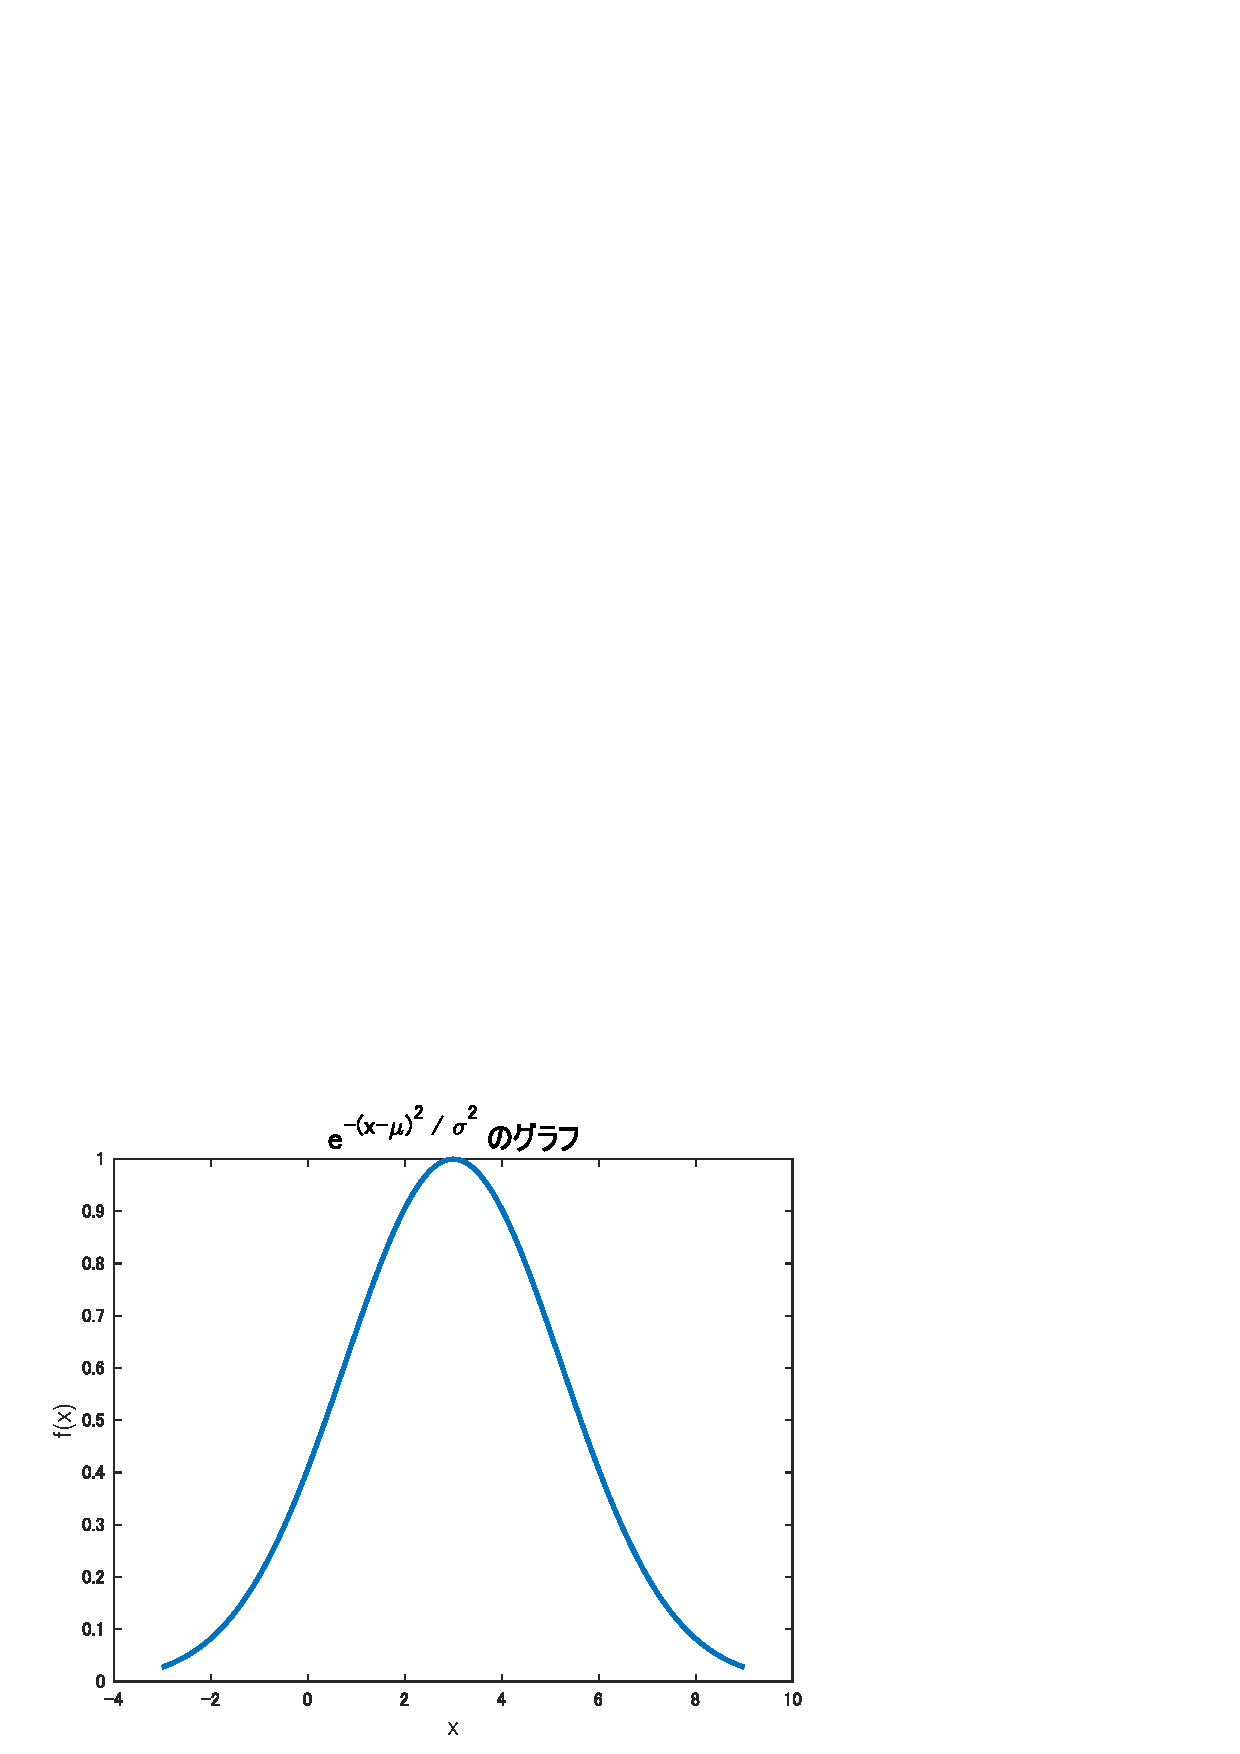
\includegraphics[width=120mm,bb=0 0 432 288]{figures/normal4.png}
  \caption{式(\ref{eq:normal4})の図.(平均3, 分散10の場合)}
\end{figure}

え?式(\ref{eq:normal})と違うじゃないかって?\\
せっかちだなぁ......余裕がない人間はモテないですよ.\\
\\
ん?僕ですか?別に同期や後輩が軒並み揃って国内/国際学会に行ってたり,  ペーパーがアクセプトされてたりするからって全然焦ってないです.もう余裕すぎてこんな同人誌書いてるくらいですもん. \\
\\
うん. これ書いたら暫く更新やめます.
\\
\\
まあ, グラフの形は実際これで完成なのです. ただ, 今我々が求めていたのは正規分布の「確率密度関数」でしたね?\\
\\
確率の密度なのですから, 当然合計して1にならないといけないわけで, 先程の式(\ref{eq:normal4})ではその点がダメなのです. ちゃんと全確率点での値を足して1になるように正規化する必要があります.\\
\\
つーわけで積分方程式を解きましょ...っとその前に, 出てくる計算結果を綺麗にするために式(\ref{eq:normal4})に細工をし, $\sigma^2$を$2\sigma^2$にしておきます. 2が付きましたが, グラフの性質自体は変わりませんね?\\
\\
では積分方程式.
\begin{eqnarray}
\int_{-\infty}^{\infty} c e^{-\frac{(x-\mu)^2}{2\sigma^2}} dx= 1
\end{eqnarray}
を解きます...出来たものがこちらです.

\begin{eqnarray}
\label{eq:c}
c = \frac{1}{\sqrt{2\pi\sigma^2}}
\end{eqnarray}

式(\ref{eq:c})で得られたcを改めて式(\ref{eq:normal4}の変形版)に代入すると

\begin{eqnarray}
f(x) = \frac{1}{\sqrt{2\pi\sigma^2}}e^{-\frac{(x-\mu)^2}{2\sigma^2}}
\end{eqnarray}

が出てきましたね!良かった良かった. 以上が正規分布の確率密度関数の導出工程でした. フーリエなんかに比べれば雑魚ですね!ワンパンでした!\\
え?積分方程式の解き方ですか?なんかMATLABにお願いしたら解いてくれました...

\subsubsection{100p\%点}
次. 正規分布を学ぶ意味は, この概念があるからといっても過言じゃない重要な性質です. 正規分布は平均が丁度真ん中で, 広がり方は分散によって定義される左右対称な特殊な分布でしたね?\\\\
つまり, 平均の周辺であるほど高確率で観測され, 裾野ほど「レア」な事象というわけです.\\\\
この性質を利用して, 正規分布には「100p\%点」と呼ばれる指標を導入する事が出来ます. これは「その点以上(以下)の部分の確率の合計がpになる境界」を指します. x軸の正方向なら上側, 負方向なら下側, 両方を指すなら両側100p\%点です. \\\\
言葉だとややこしいですが, グラフで見れば一瞬で分かります.


\begin{figure}[H]
\label{im:upper}
  \centering
  \includegraphics[width=120mm,bb=0 0 432 288]{figures/upper_p.png}
  \caption{正規分布の上側5\%点}
\end{figure}

\begin{figure}[H]
\label{im:bilateral}
  \centering
  \includegraphics[width=120mm,bb=0 0 432 288]{figures/bilateral_p.png}
  \caption{正規分布の両側5\%点}
\end{figure}

上側5\%に比べ, 両側5\%は左右に領域が分散した分上側の領域が狭くなってるのに注意です. \\
\\
だいたい, 正規分布でよく用いられるのは上下両側の5\%と1\%点です. 何に使うのかはあとで説明するので, ひとまず概念だけ覚えておいてください.

\subsection{t分布}
少ない標本数をもとに母分散がわかっていない母集団の母平均推定に使われるのがt分布です. 詳しくは推定の項で触れるので, ここでは確率密度関数と性質の確認をします.

\begin{eqnarray}
\label{eq:student}
f(x) = k(1 + \frac{x^2}{\alpha})^{-\frac{\alpha+1}{2}}
\end{eqnarray}

式(\ref{eq:student})がt分布の確率密度関数です. ここで$k$は定数, $\alpha$は自由度という指標で, この形を「自由度$\alpha$のt分布」と表現します. 自由度とは何かはここでは説明しませんが, 母集団によって算出できる値です. それ以外の部分では正規分布に似ていますね. 実際, 自由度$\alpha$が十分に大きい場合には正規分布になります. ただこいつの平均と分散は

\begin{eqnarray}
\mathbb{E}(X) = 0\\
\mathbb{V}(X) = \frac{\alpha}{\alpha-2}
\end{eqnarray}
です. 

\begin{figure}[H]
\label{im:student}
  \centering
  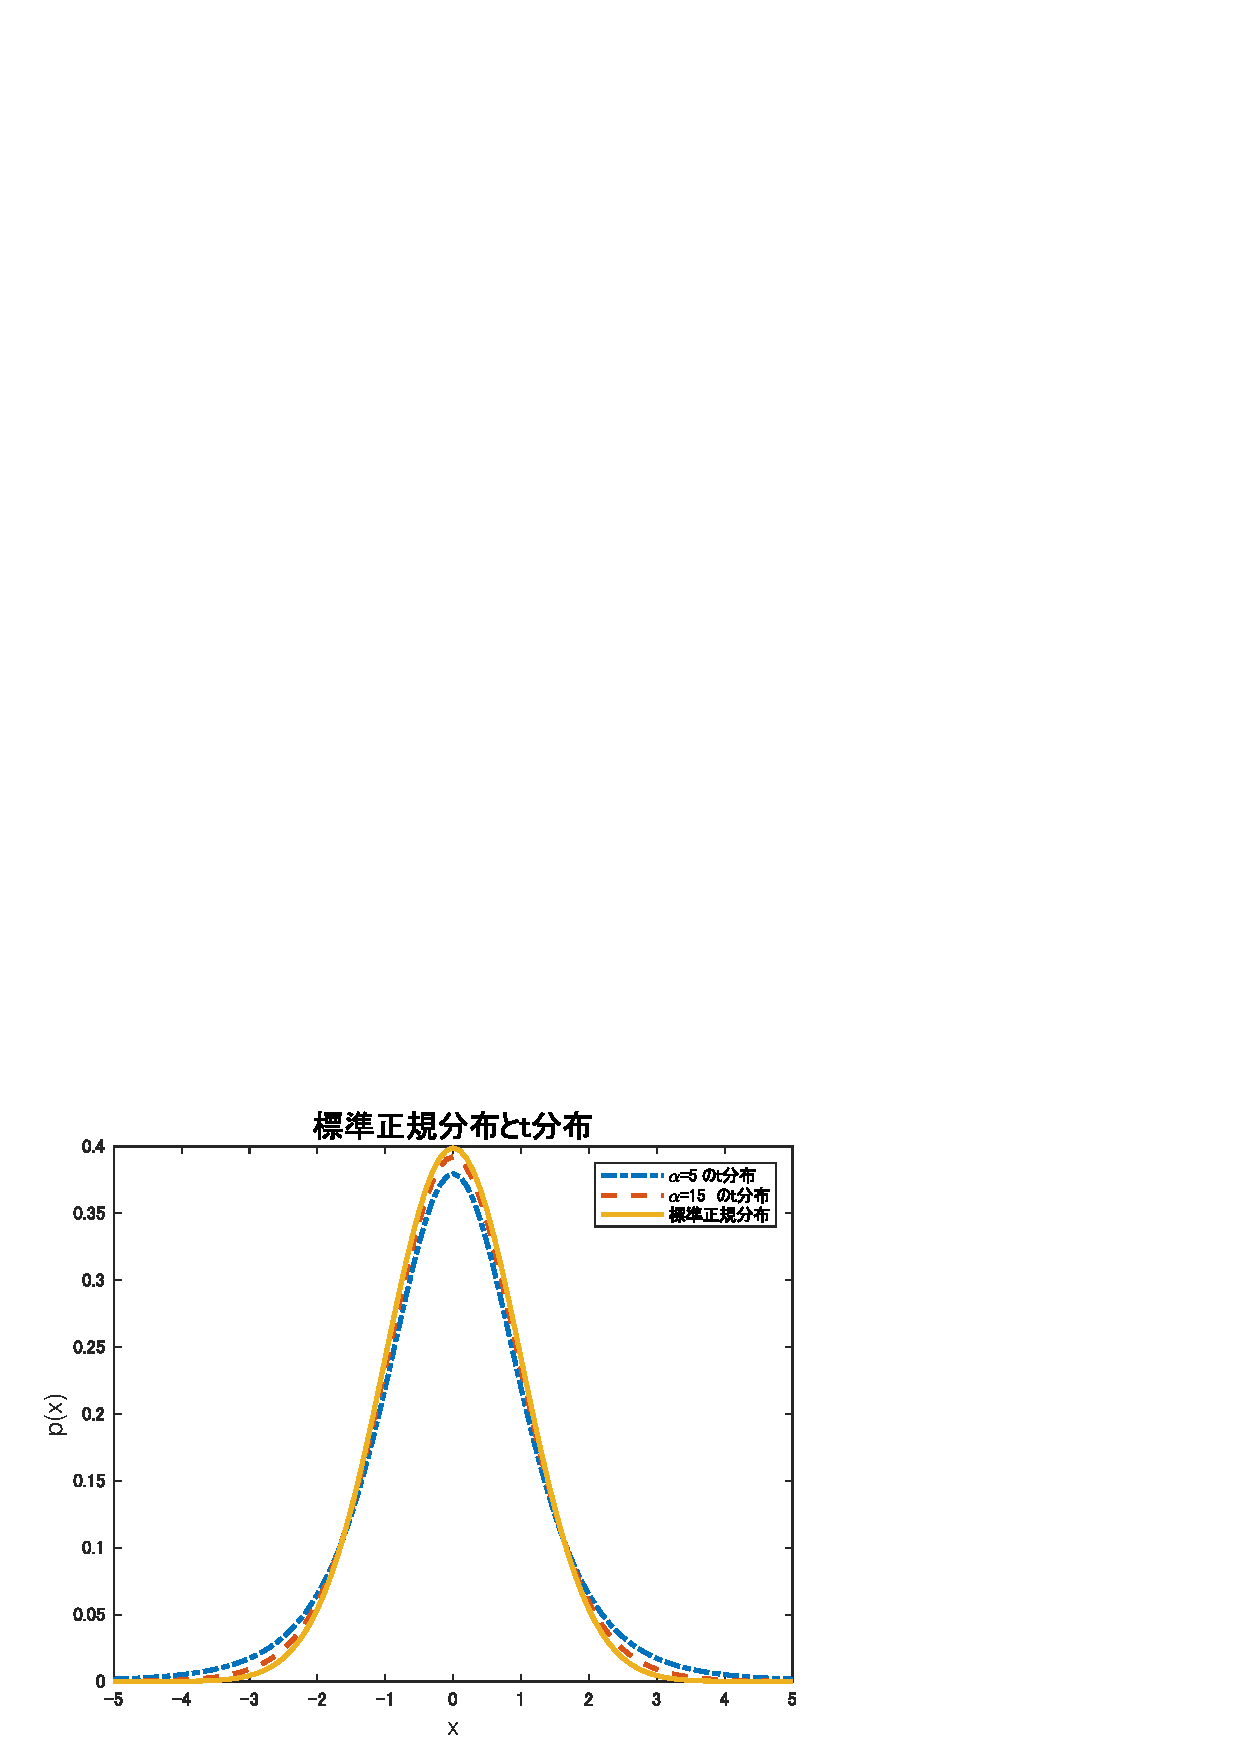
\includegraphics[width=120mm,bb=0 0 432 288]{figures/student.png}
  \caption{自由度の異なるt分布と標準正規分布}
\end{figure}
自由度の異なるt分布と標準正規分布の比較です. 標準正規分布とは, 正規分布のうち平均が0, 分散が1のやつです. $\alpha$の値が大きいとほぼ同じ形になる事が分かると思います.\\
\\
では何に使うのかですが, そこはひとまず置いておきます. とにかくこういう分布があるのです.


\subsection{F分布}
F分布は, 少し特殊な形をしていますが非常に重要です. どう重要かというとF分布はこれまでの分布と異なり, 2つの母集団から得られた標本分散の比の確率分布になります. これの何がすごいのかというと, 例えば図(\ref{im:f_dist})は自由度が3の母集団Aと自由度が10の母集団BのF分布ですが, 「普通は」この組み合わせだと0から2あたりの値になる事が多いのです. \\
\\
しかしもし今, 自由度3と10のとある母集団A,B間でF値を取ったら6とかが出たとします. \\
通常はありえない値, つまり統計的に考えると「自由度だけでなく分散そのものに差がある = A,Bの母集団は異なる」となるわけですね. こちらも詳しくは後程. 式はえぐえぐです. 震えろ.

\begin{eqnarray}
f(x) = \frac{kx^{\frac{m}{2}-1}}{\{1 + (\frac{m}{n})x\}^{\frac{m+n}{2}}}
\end{eqnarray}

こいつの導出はいいです. 僕もわからん. 気が向いたら勉強してまとめるかも. 例によってkは定数, m,nは標本集団2つのそれぞれの自由度です. こいつは「自由度m,nのF分布」と表現されます. 今はそれだけ. 続いてグラフです. 幸いこっちは簡単.

\begin{figure}[H]
\label{im:f_dist}
  \centering
  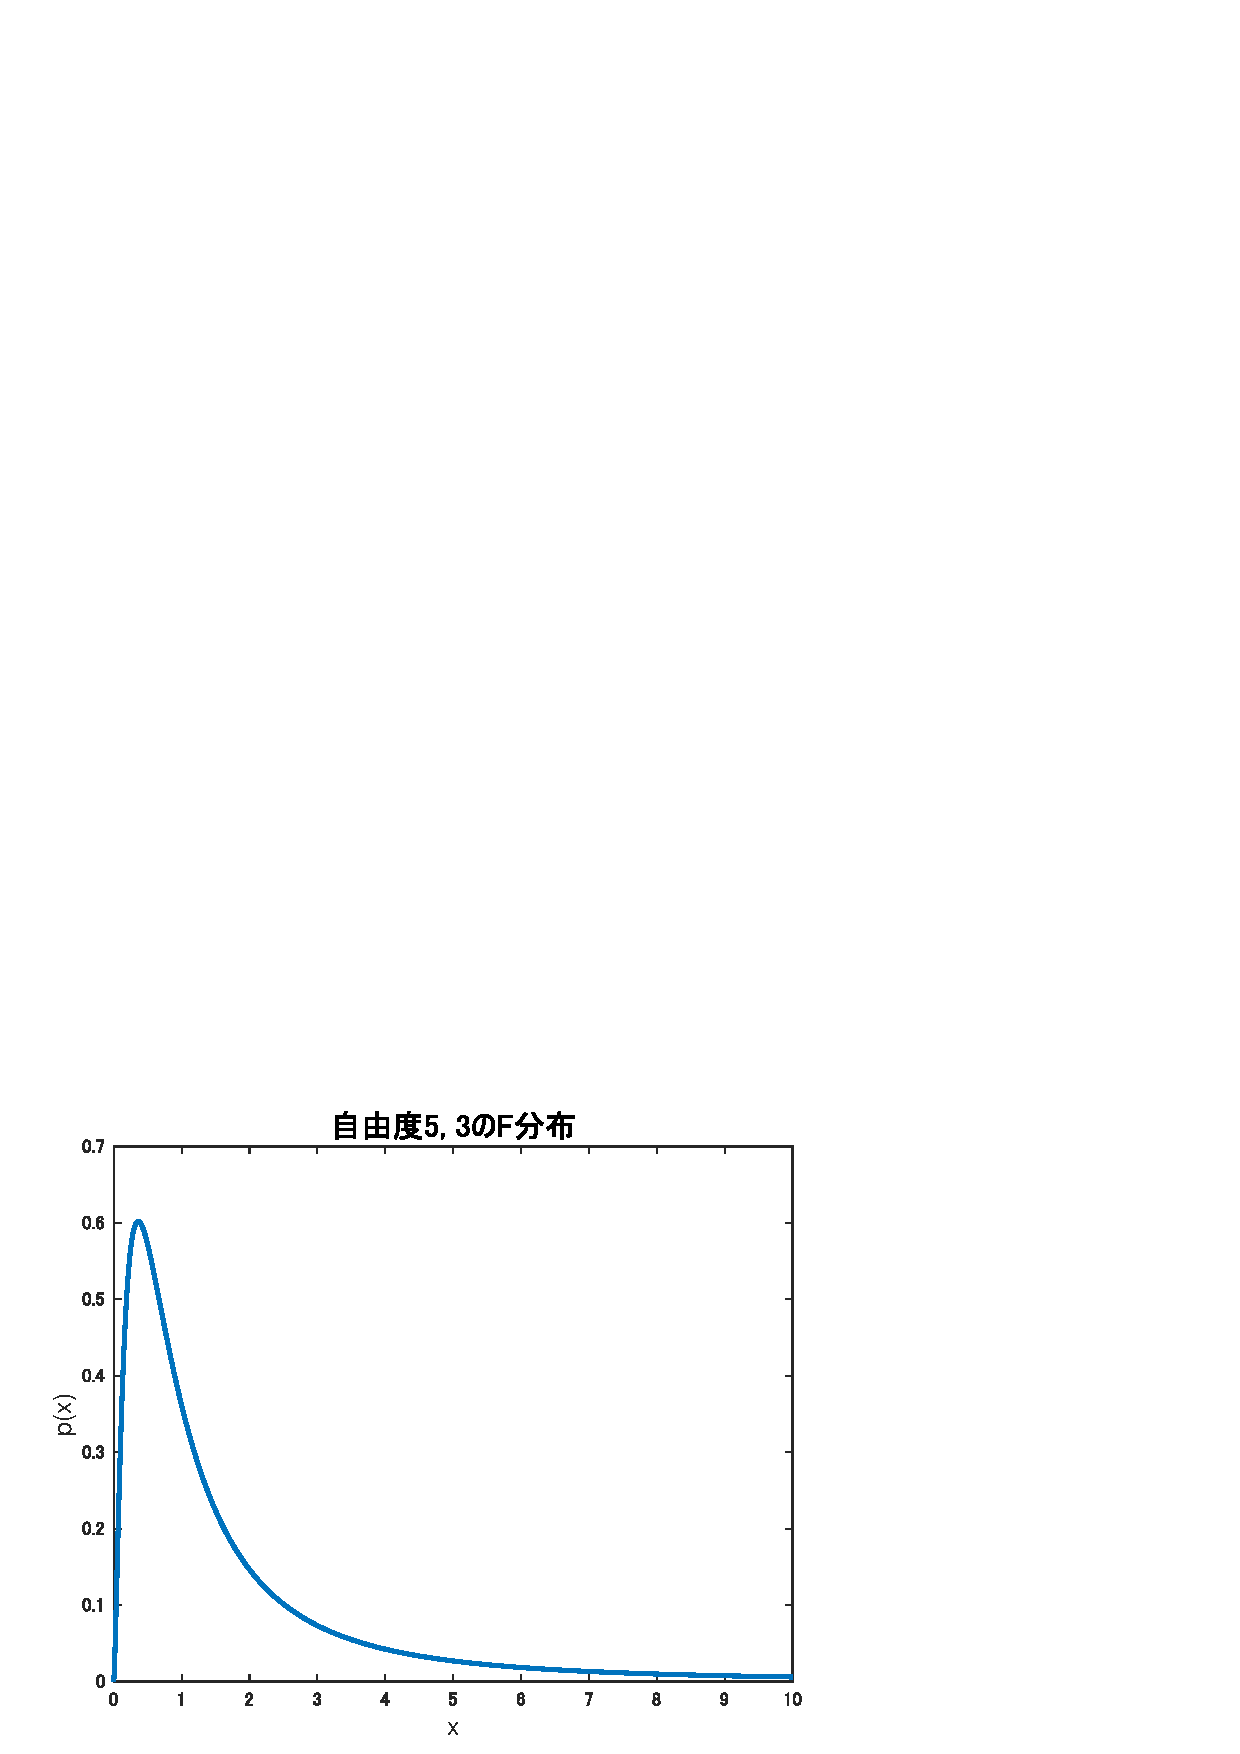
\includegraphics[width=120mm,bb=0 0 432 288]{figures/f_dist.png}
  \caption{自由度3.10のF分布}
\end{figure}

恒例の平均値と分散です. こいつらも殺意高めだけど覚える必要は今のところ皆無だと思ってます.

\begin{eqnarray}
\mathbb{E}(X) = \frac{n}{n-2}\\
\mathbb{V}(X) = \frac{2n^2 (m+n-2)}{m(n-2)^2(n-4)}
\end{eqnarray}

\subsection{$\chi^2$分布}
ラスト. $\chi^2$分布です. こいつも重要です. 我々は結果を理論に落とし込む時, なんらかの数式に近似したり回帰したりするわけですが, 実際問題理論と観測値が完全に一致するなんていう事はまれで, 様々な要因で若干の誤差が生じます. その誤差が「誤差」なのか「理論の誤り」なのかを評価する時に使うのがこの分布とそれに基づく検定です. \\
\\
式はこちらです. 
\begin{eqnarray}
f(x) = k\chi^{\frac{\alpha}{2}-1}e^{-\frac{\chi}{2}}
\end{eqnarray}

またえぐえぐですね. えぐえぐと言えば, 筆者は声優の江口拓也さんが「やはり俺の青春ラブコメは間違っている」のラジオでやっていた「ぼっちラジオ」が大好きです. どうせこんな数学の同人誌読んでる人は陰キャだし, 楽しめると思います. 是非YouTubeで検索してみてください.\\
\\
さて, 例によってここの$\alpha$は自由度, kは定数です.\\
幸い, どこの説明を見てもこの式は使わないと言われているので覚えなくていいでしょう.\\
\\
平均値と分散です.
\begin{eqnarray}
\mathbb{E}(X) = \alpha \\
\mathbb{V}(X) = 2\alpha
\end{eqnarray}
簡単すぎワロタww\\
ついでグラフです.


\begin{figure}[H]
\label{im:chi}
  \centering
  \includegraphics[width=120mm,bb=0 0 432 288]{figures/kai.png}
  \caption{自由度の異なる$\chi^2$分布}
\end{figure}
 こいつは結構F分布に似てますね. ただ注意が必要なのは, F分布は標本分散の比に関する分布ですが$\chi^2$分布は標本分散そのものの分布です.

\newpage
\section{統計的推定}

\subsection{サンプリングとは}
\subsection{中心極限定理}
\subsection{普遍分散}
\subsection{点推定}
\subsection{区間推定}
\subsubsection{信頼度/信頼区間/100p\%点}

\section{統計的検定}
\subsection{仮説検定と有意差}
\subsection{母平均の変化の検定}
\subsubsection{母分散既知}
\subsubsection{母分散未知}
\subsubsection{十分に大きい標本の場合}
\subsection{母比率の変化の検定}
\subsection{母平均の違いの検定}
\subsection{母分散の違いの検定}
\subsection{母比率の違いの検定}
\subsection{第一種/第二種の過誤}

\section{分散分析}
\subsection{分散分析とは}
\subsubsection{因子と水準}
\subsubsection{n元配置の分散分析}
\subsubsection{分散分析の繰り返し}
\subsection{一元配置の分散分析}
\subsection{二元配置の分散分析}
\subsection{繰り返しのある二元配置の分散分析}
\section{回帰分析}
\end{document}